\section{High level Architecture}
In the following section we present the high level architecture underlying our solution. Therefore, we take into account each component individually. Once introduced the architecture, we provide an overview on the main interactions taking place between the introduced components.
\subsection{Main components}
\label{fig:architecture_diagram}
\begin{figure}[t]
\centering
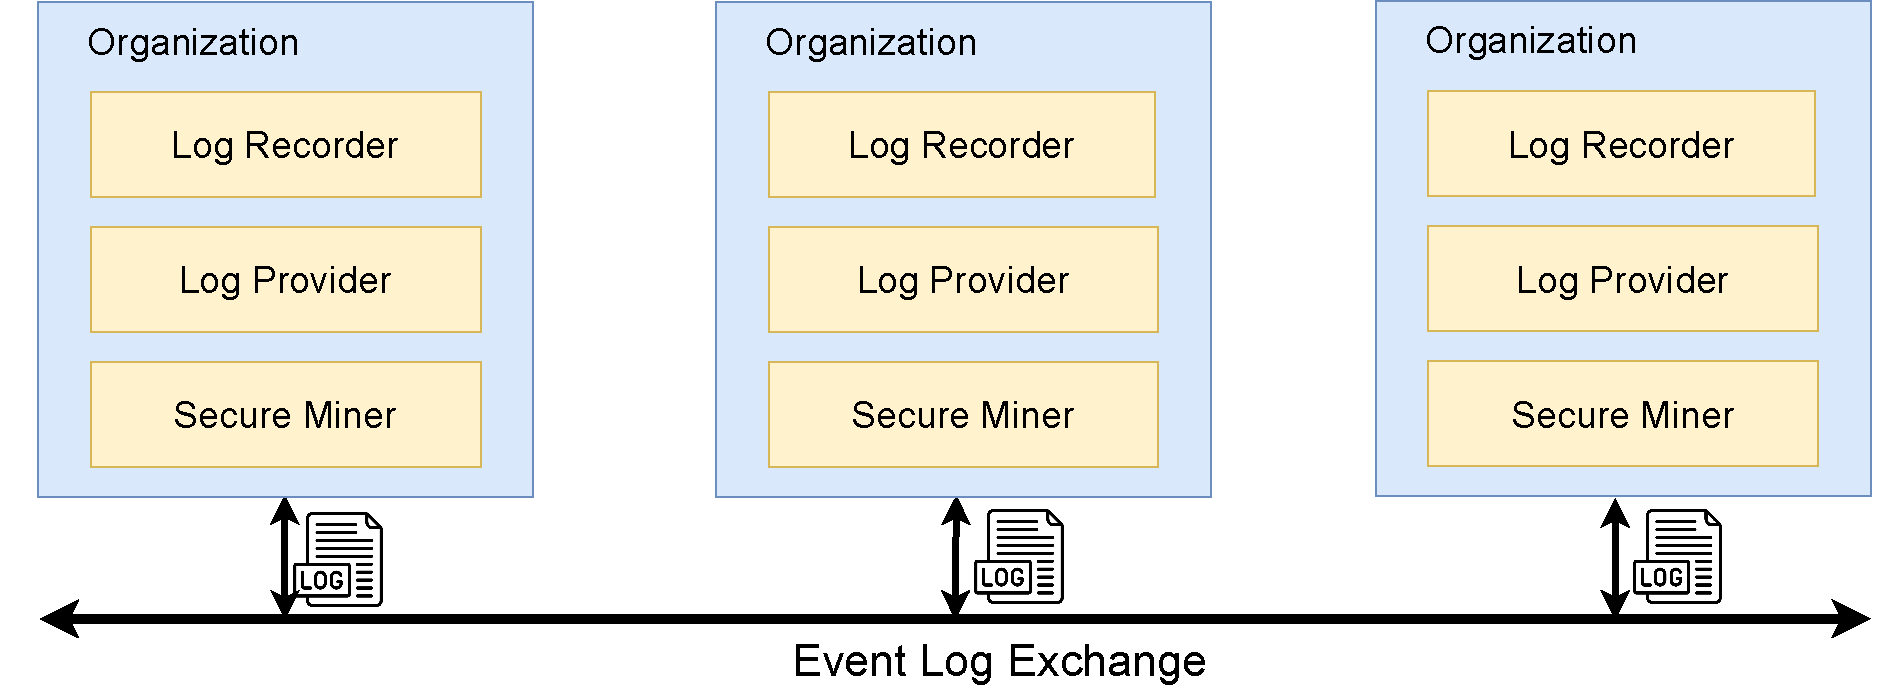
\includegraphics[width=10cm]{content/figures/architecture_diagram.pdf}
\caption{High-level architectural overview of the framework.}
\label{fig:implementation}
\end{figure}
Our architecture involve networks of nodes controlled by different \texttt{Organization}s exchanging their event logs. \texttt{Organization}s in the same network collaborate to reach a common objective sharing one or more business processes. Each organization is associated with  The Hospital and Specialized Clinic, mentioned in the running example, provide an example of partner organizations.

In \cref{fig:architecture_diagram}, we propose an high level schematization of our solution. Each organization embeds three main components: the \texttt{EMS Interface}, the \texttt{Log Provider} and the \texttt{Trusted Miner}. %collects the logic to interact with the Environmental Management System (EMS) of the organization. The \texttt{Log Provider} component deliver on-demand data to partner organization's systems. The \texttt{Trusted Miner} executes process mining algorithms inside the \texttt{Trusted Execution Environment} using event log retrieved from partner organizations.
In the next paragraph, we address the newly mentioned components.
\subsubsection{ERP Interface}
The \texttt{ERP Interface} collects the logic to interact with the Enterprise Resource Planning (ERP) system  of the \texttt{Organization}. ERP systems helps organizations to
handle business processes including accounting and resource management. The mantainance of event logs is one of the many tasks performed by these systems. In our architecture, we generalize the interaction with these systems through the \texttt{ERP Interface}. The \texttt{ERP Interface} provide the local \texttt{Log Provider} and \texttt{Trusted Miner} access to event logs generated inside the \texttt{Organization}.
\subsubsection{Log Provider}
The \texttt{Log Provider} component deliver on-demand data to \texttt{Trusted Miner} components belonging to partner \texttt{Organization}'s. It handle event log request through access control methodologies, thanks to which the identity of the sender is determined. \texttt{Log Provider}s authenticate event log requests using asymetric encryption methodologies. Through the latter, \texttt{Log Provider}s verifiy parameters embedded in the data request. When provisioning data, the \texttt{Log Provider} retrieve the local event log communicating with the \texttt{ERP Interface}.

\subsubsection{Trusted Miner}
 The \texttt{Trusted Miner} executes process mining algorithms inside the \texttt{Trusted Execution Environment} using local event log and event log retrieved from partner organizations.
\subsection{Workflow}
\subsubsection{Initialization}
\subsubsection{Data Exchange}
\subsubsection{Data Elaboration}



